
\newpage{}
\section{Calibración}
	\subsection{Herramienta necesaria}
		\begin{itemize}
			\item Calibre digital.
		\end{itemize}
	\subsection{Calibración eje X}
		Una vez que tenemos montada nuestra impresra, el siguiente paso que haremos será el de calibrar los motores de odos los ejes para que se muevan la distancia que nosotros le indicamos.
		Para ello nos conectaremos con pronterface a nuestra impresora.\\
		
		Colocaremos el calibre como se muestra en la figura ~\ref{fig:1.calibracion}. Una vez que está colocado en una posición fija, fíjaremos la medida del calibre a 0,00, para que tome como el origen de medidas esa posición, una vez fijada, en pronterface le mandaremos mover 100mm. Una vez que termine de moverse, comprobaremos cuanto se ha movido en realidad y apuntamos ese valor.\\
		\begin{figure}[H]
		        \centering
		        \begin{subfigure}[htb]{0.4\textwidth}
		                \centering
		                \includegraphics[width=\textwidth]{../../Fotos/111.jpg}
		                
		                %\label{fig:agujero.tapado}
		        \end{subfigure}
		        \begin{subfigure}[htb]{0.4\textwidth}
		                \centering
		                \includegraphics[width=\textwidth]{../../Fotos/112.jpg}
		                
		                %\label{fig:agujero.pasante}
		        \end{subfigure}
		        \caption{Calibración eje X}\label{fig:1.calibracion}
		\end{figure}
		Llegados a este punto, necesitaremos abrir nuestro marlin, e irnos al fichero Coniguration.h, sobre la línea 218, debemos buscar la configuración como se muestra en la figura 
~\ref{fig:2.calibracion}.\\	
		\begin{figure}[!htp]
			\centering
			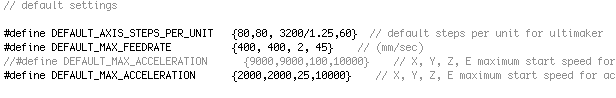
\includegraphics[width=0.8\textwidth]{../../Fotos/119.png}
			\caption{Configuración Marlin}
			\label{fig:2.calibracion}
		\end{figure}
		
		Cada parámetro está en el siguiente orden: define DEFAULT AXIS STEPS PER UNIT  (X,Y,Z,EXTRUSOR).Ahora necesitaremos hacer una regla de tres simple.\\

			\begin{equation}\label{eq:calibracion}
			\mbox{pasos deseados}=  \frac{10*\mbox{pasos actuales}}{\mbox{medida real}}
			\end{equation}

		Donde "Pasos actuales" pondremos el valor que tengamos en marlin y en "medida real", la medida que acabamos de medir, una vez que obtenemos "pasos deseados" lo cambiamos en marlin, compilamos y volvemos a transferir el programa a la tarjeta.Deberemos repetir esta operativa hasta conseguir un valor lo más aproximado a 10.00 con el calibre.
		
		\subsection{Calibración eje Y}
		La operativa es la misma que vimos en el eje X lo único que cambia es la posición donde poner el calibre, se muestra en la figura ~\ref{fig:3.calibracion}
		\begin{figure}[H]
		        \centering
		        \begin{subfigure}[htb]{0.4\textwidth}
		                \centering
		                \includegraphics[width=\textwidth]{../../Fotos/113.jpg}
		                
		                %\label{fig:agujero.tapado}
		        \end{subfigure}
		        \begin{subfigure}[htb]{0.4\textwidth}
		                \centering
		                \includegraphics[width=\textwidth]{../../Fotos/114.jpg}
		                
		                %\label{fig:agujero.pasante}
		        \end{subfigure}
		        \caption{Calibración eje Y}\label{fig:3.calibracion}
		\end{figure}
		\subsection{Calibración eje Z}
		La operativa es la misma que vimos en el eje X lo único que cambia es la posición donde poner el calibre, se muestra en la figura ~\ref{fig:4.calibracion}
		\begin{figure}[H]
		        \centering
		        \begin{subfigure}[htb]{0.4\textwidth}
		                \centering
		                \includegraphics[width=\textwidth]{../../Fotos/115.jpg}
		                
		                %\label{fig:agujero.tapado}
		        \end{subfigure}
		        \begin{subfigure}[htb]{0.4\textwidth}
		                \centering
		                \includegraphics[width=\textwidth]{../../Fotos/116.jpg}
		                
		                %\label{fig:agujero.pasante}
		        \end{subfigure}
		        \caption{Calibración eje Z}\label{fig:4.calibracion}
		\end{figure}
		
		\subsection{Calibración extrusor}
		Para terminar con el proceso de calibración pasaremos al extrusor. Para ello, haremos una marca en el filaeto de plástico que hemos introducido previamente en el extrusor. La marca tiene que estar lo suficientemente alejado del extrusor como para que recorra 1Omm. Una vez hecha la muesca, reseteamos el valor del calibre para que esa sea la posición 0,00(ver figura ~\ref{fig:3.calibracion}). En pronterface, le damos a extruir 10mm y vemos lo que ha recorrido el plástico. Apuntamos ese valor y volvemos a calcular los pasos que debemos configurar en nuestro firmare con ayuda de la ecuación \ref{eq:calibracion} 
		\begin{figure}[H]
		        \centering
		        \begin{subfigure}[htb]{0.4\textwidth}
		                \centering
		                \includegraphics[width=\textwidth]{../../Fotos/117.jpg}
		                
		                %\label{fig:agujero.tapado}
		        \end{subfigure}
		        \begin{subfigure}[htb]{0.4\textwidth}
		                \centering
		                \includegraphics[width=\textwidth]{../../Fotos/118.jpg}
		                
		                %\label{fig:agujero.pasante}
		        \end{subfigure}
		        \caption{Calibración eje extrusor}\label{fig:5.calibracion}
		\end{figure}